In this section the overall design of the application will be detailed, specifically in regards to the initial requirements specification. In addition more detail will be discussed on the desired functionality for all aspects of the application from which a paper prototype will be constructed and evaluated as a goal for the final submission.

\subsection{Initial Concept}
The initial concept for the project was to construct an application that utilized the multiple, accessible screens in the learning zone. Each screen would display balloons which could ``float'' between them in a circular fashion. In addition, users would be able to interact with one or more balloons by waving their hands in a manner to ``push'' the balloons a certain way. There would be various types of balloons, from those displaying content from twitter feeds or user uploaded content, to simple ``customizable'' balloons that had no content.

Each balloon could be dropped into one of several paint buckets along the bottom of the screen in order to ``paint'' them a certain colour or pattern, and content balloons could be burst to reveal the full content inside. When burst, content would be displayed on a window in front of the screen for some time before disappearing on its own or being closed by the user. The content itself would be updated regularly as users uploaded their own content or the twitter feed updates, from which a particular number of each kind of balloon would be maintained at all times. In terms of the content, it would be either a series of twitter feeds which could provide the user with useful information or a custom content balloon which displayed desired text and graphic, all chosen by a user. A QR code would be provided for all balloons in order to allow the user to access the original source through the use of a QR Code reader on a smartphone. A later iteration brought forward the use of a rating system which would allow users to rate user content balloons which would then be affect their priority level and frequency on the screen.

Lastly, the application would incorporate a web client for users to submit their own content to be displayed on the screens on a balloon. It would allow users to enter in their desired text, provide a picture and web link, and customize their balloon's colour. In addition, their would be a moderator interface implemented within that would allow chosen users to delete any inappropriate content as filters were not to be considered as requested by the client.

\begin{center}
\textit{Please note that additional features were implemented over the course of the project but will not be detailed until later in the evaluation section of the report. This is because all extra requirements were constructed from user feedback.}
\end{center}

\subsection{Desired Functionality}
As the balloons are the main focus of the application, the abstract functionality will be considered as such; balloons must be created, displayed, and destroyed. In terms of creation, this will come about through the periodic updates of the twitter system and user content system. After being displayed on a random screen, the balloons must have the ability to transition onto another screen if one should reach the edge of its current screen. Finally, destruction of a balloon will occur when a user ``pops'' it or when the next patch of updates comes through; which will destroy all the current balloons. A maximum number of seven balloons will be loaded onto each screen, totaling twenty one balloons in total for three screens.

Each balloon had to serve two functions: being customizable and being interactive (the ability to be moved and burst). Customizing a balloon would happen by pushing it into a paint bucket, and depending on the kind of paint bucket involved, would react appropriately. There would be three buckets for each primary colour, allowing balloons to be dipped into multiple buckets and be blended (for example dipping a balloon into a red bucket and then a blue bucket would result in a purple balloon). In addition two pattern paint buckets (strips and spots) would exist and would provide an overlay to the balloon. Patterns would have a toggle setting, meaning the user could have no pattern by hitting the same bucket again.

Secondly, balloons would burst to reveal a more detailed view of their content. This view would appear like a secondary window over the main screen (but not taking up a high percentage of the available screen such that the background could not be seen) and after 30 seconds would disappear on its own. Optionally, a user may close the box early through the use of a red ``X'' in the corner of the screen. These content boxes would display their summary text along the top, their full text in the middle, and an image and QR code representing a URL to the original source. In the case of twitter content, the full text would be the entire tweet, the image would be the twitter account's user profile and the URL would simply link to the tweet itself. In the case of custom user content, the text, image and URL would all be as specified by the user through a separate web interface. Finally the screens needed to be able to communicate with each other to allow balloons to ``pass through'' with the appropriate information.

With regards to the rating system, the QR codes for custom user content would firstly redirect to an interim page on a user's phone that would allow the user to vote the content up or down (or not at all) before visiting the specified URL. This would then help better rated content appear more frequently over more badly rated content.

In terms of the web application, a user would be able to login with their MACS user name and password. All current user content would be displayed in a list format from which the user could access the information independently. In addition, a user would then be able to create their own content, which would then be added to the custom content system for possible selection. The administrative side of the application would only require the list of content with an additional delete option.

\subsubsection{Kinect}
In order to utilize the playful nature of the Kinect, and to encourage new users to pick up the concepts quickly, interaction with the application needed to be achieved in the most intuitive and simple way possible. The solution to this was to make the balloons physical entities that users are able to hit and push as desired. This one concept facilitates all functions - users customize balloons by pushing them into paint buckets, and burst balloons by squeezing them between their hands. The one exception to this is the close button on the content window, which is activated by a user hovering their hand over the button for a small length of time - a gesture which is frequently used in native Microsoft Kinect applications for menu selection.

\subsubsection{Twitter}
Content would be received from the university's Twitter account to ensure content that is relevant to the users of the learning zone is displayed. This would not be filtered and would be selected for display based on age where the newest content comes first.

\subsubsection{User Uploads}
Users would be able to upload their own custom content to be displayed as a balloon. Using an additional interface accessed through a web page a user would be able to define summary text to be displayed on the small boxes carried by the balloons, full text as displayed on the content window, an image to be displayed on the content window, a URL that the QR code will allow smartphone users to visit and the colour and pattern of their specific balloon. Using this, a user would be able to see their personal balloon on the screen displaying their student or research work as the original applications in the learning zone had facilitated.

\subsection{Presentation}
With the application utilizing the Kinect and exhibiting a playful nature, a cartoon-like style was chosen to encourage play from its users. Bold primary colours and a simple art style were chosen in order to maintain the light-hearted feel of the learning zone as well as provide something pleasing to the eye when not in use. Balloons blown by a gentle breeze in addition to a bright blue sky with fluffy clouds were chosen to promote a relaxing atmosphere, in addition to comical paint buckets.

Design patterns were referenced for the layout of the interface, keeping all customization tools along the bottom of the screen and fully maximizing screen space for the balloons by partially hiding the paint buckets when no balloons are nearby. 

\subsection{Scope, Limitations and Assumptions}
As no preliminary research was conducted before the start of the design, but was carried out during it, accessibility was not considered for the application. A number of Kinect limitations were discovered but as these were a hardware disability, they are located under the appropriate heading for future evaluation. In addition, sound and visual cues were not implemented but were investigated and will also be included within the future work section of the report.

\subsection{Paper Prototype}
A paper prototype was constructed to demonstrate one screen of the application's design to the client. It showed user interactivity, in relation to balloon customization, including the movement of the paint buckets and the bursting of balloons to reveal content. In addition it demonstrated two different approaches to displaying balloons - on their own or as carrying boxes with summary text for each piece of content - the latter of which was chosen by the client. The paper prototype received positive feedback and incorporated all desired functionality and thus was the basis for the software design that was to follow.

\begin{figure}[h]
\begin{centering}
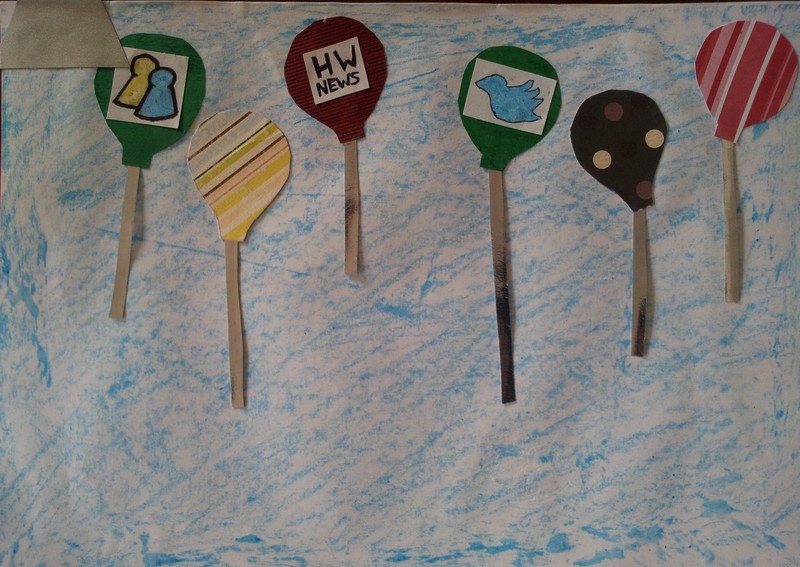
\includegraphics[width=\textwidth]{Diagrams/PaperPrototype.jpg}
\par\end{centering}

\caption{Paper Prototype}
\label{PaperPrototype}
\end{figure}
